
%% bare_conf.tex
%% V1.3
%% 2007/01/11
%% by Michael Shell
%% See:
%% http://www.michaelshell.org/
%% for current contact information.
%%
%% This is a skeleton file demonstrating the use of IEEEtran.cls
%% (requires IEEEtran.cls version 1.7 or later) with an IEEE conference paper.
%%
%% Support sites:
%% http://www.michaelshell.org/tex/ieeetran/
%% http://www.ctan.org/tex-archive/macros/latex/contrib/IEEEtran/
%% and
%% http://www.ieee.org/

%%*************************************************************************
%% Legal Notice:
%% This code is offered as-is without any warranty either expressed or
%% implied; without even the implied warranty of MERCHANTABILITY or
%% FITNESS FOR A PARTICULAR PURPOSE! 
%% User assumes all risk.
%% In no event shall IEEE or any contributor to this code be liable for
%% any damages or losses, including, but not limited to, incidental,
%% consequential, or any other damages, resulting from the use or misuse
%% of any information contained here.
%%
%% All comments are the opinions of their respective authors and are not
%% necessarily endorsed by the IEEE.
%%
%% This work is distributed under the LaTeX Project Public License (LPPL)
%% ( http://www.latex-project.org/ ) version 1.3, and may be freely used,
%% distributed and modified. A copy of the LPPL, version 1.3, is included
%% in the base LaTeX documentation of all distributions of LaTeX released
%% 2003/12/01 or later.
%% Retain all contribution notices and credits.
%% ** Modified files should be clearly indicated as such, including  **
%% ** renaming them and changing author support contact information. **
%%
%% File list of work: IEEEtran.cls, IEEEtran_HOWTO.pdf, bare_adv.tex,
%%                    bare_conf.tex, bare_jrnl.tex, bare_jrnl_compsoc.tex
%%*************************************************************************

% *** Authors should verify (and, if needed, correct) their LaTeX system  ***
% *** with the testflow diagnostic prior to trusting their LaTeX platform ***
% *** with production work. IEEE's font choices can trigger bugs that do  ***
% *** not appear when using other class files.                            ***
% The testflow support page is at:
% http://www.michaelshell.org/tex/testflow/



% Note that the a4paper option is mainly intended so that authors in
% countries using A4 can easily print to A4 and see how their papers will
% look in print - the typesetting of the document will not typically be
% affected with changes in paper size (but the bottom and side margins will).
% Use the testflow package mentioned above to verify correct handling of
% both paper sizes by the user's LaTeX system.
%
% Also note that the "draftcls" or "draftclsnofoot", not "draft", option
% should be used if it is desired that the figures are to be displayed in
% draft mode.
%
\documentclass[conference]{IEEEtran}
% Add the compsoc option for Computer Society conferences.
%
% If IEEEtran.cls has not been installed into the LaTeX system files,
% manually specify the path to it like:
% \documentclass[conference]{../sty/IEEEtran}





% Some very useful LaTeX packages include:
% (uncomment the ones you want to load)


% *** MISC UTILITY PACKAGES ***
%
%\usepackage{ifpdf}
% Heiko Oberdiek's ifpdf.sty is very useful if you need conditional
% compilation based on whether the output is pdf or dvi.
% usage:
% \ifpdf
%   % pdf code
% \else
%   % dvi code
% \fi
% The latest version of ifpdf.sty can be obtained from:
% http://www.ctan.org/tex-archive/macros/latex/contrib/oberdiek/
% Also, note that IEEEtran.cls V1.7 and later provides a builtin
% \ifCLASSINFOpdf conditional that works the same way.
% When switching from latex to pdflatex and vice-versa, the compiler may
% have to be run twice to clear warning/error messages.






% *** CITATION PACKAGES ***
%
%\usepackage{cite}
% cite.sty was written by Donald Arseneau
% V1.6 and later of IEEEtran pre-defines the format of the cite.sty package
% \cite{} output to follow that of IEEE. Loading the cite package will
% result in citation numbers being automatically sorted and properly
% "compressed/ranged". e.g., [1], [9], [2], [7], [5], [6] without using
% cite.sty will become [1], [2], [5]--[7], [9] using cite.sty. cite.sty's
% \cite will automatically add leading space, if needed. Use cite.sty's
% noadjust option (cite.sty V3.8 and later) if you want to turn this off.
% cite.sty is already installed on most LaTeX systems. Be sure and use
% version 4.0 (2003-05-27) and later if using hyperref.sty. cite.sty does
% not currently provide for hyperlinked citations.
% The latest version can be obtained at:
% http://www.ctan.org/tex-archive/macros/latex/contrib/cite/
% The documentation is contained in the cite.sty file itself.






% *** GRAPHICS RELATED PACKAGES ***
%
\ifCLASSINFOpdf
  % \usepackage[pdftex]{graphicx}
  % declare the path(s) where your graphic files are
  % \graphicspath{{../pdf/}{../jpeg/}}
  % and their extensions so you won't have to specify these with
  % every instance of \includegraphics
  % \DeclareGraphicsExtensions{.pdf,.jpeg,.png}
\else
  % or other class option (dvipsone, dvipdf, if not using dvips). graphicx
  % will default to the driver specified in the system graphics.cfg if no
  % driver is specified.
  % \usepackage[dvips]{graphicx}
  % declare the path(s) where your graphic files are
  % \graphicspath{{../eps/}}
  % and their extensions so you won't have to specify these with
  % every instance of \includegraphics
  % \DeclareGraphicsExtensions{.eps}
\fi
% graphicx was written by David Carlisle and Sebastian Rahtz. It is
% required if you want graphics, photos, etc. graphicx.sty is already
% installed on most LaTeX systems. The latest version and documentation can
% be obtained at: 
% http://www.ctan.org/tex-archive/macros/latex/required/graphics/
% Another good source of documentation is "Using Imported Graphics in
% LaTeX2e" by Keith Reckdahl which can be found as epslatex.ps or
% epslatex.pdf at: http://www.ctan.org/tex-archive/info/
%
% latex, and pdflatex in dvi mode, support graphics in encapsulated
% postscript (.eps) format. pdflatex in pdf mode supports graphics
% in .pdf, .jpeg, .png and .mps (metapost) formats. Users should ensure
% that all non-photo figures use a vector format (.eps, .pdf, .mps) and
% not a bitmapped formats (.jpeg, .png). IEEE frowns on bitmapped formats
% which can result in "jaggedy"/blurry rendering of lines and letters as
% well as large increases in file sizes.
%
% You can find documentation about the pdfTeX application at:
% http://www.tug.org/applications/pdftex





% *** MATH PACKAGES ***
%
%\usepackage[cmex10]{amsmath}
% A popular package from the American Mathematical Society that provides
% many useful and powerful commands for dealing with mathematics. If using
% it, be sure to load this package with the cmex10 option to ensure that
% only type 1 fonts will utilized at all point sizes. Without this option,
% it is possible that some math symbols, particularly those within
% footnotes, will be rendered in bitmap form which will result in a
% document that can not be IEEE Xplore compliant!
%
% Also, note that the amsmath package sets \interdisplaylinepenalty to 10000
% thus preventing page breaks from occurring within multiline equations. Use:
%\interdisplaylinepenalty=2500
% after loading amsmath to restore such page breaks as IEEEtran.cls normally
% does. amsmath.sty is already installed on most LaTeX systems. The latest
% version and documentation can be obtained at:
% http://www.ctan.org/tex-archive/macros/latex/required/amslatex/math/





% *** SPECIALIZED LIST PACKAGES ***
%
\usepackage{algorithmic}
% algorithmic.sty was written by Peter Williams and Rogerio Brito.
% This package provides an algorithmic environment fo describing algorithms.
% You can use the algorithmic environment in-text or within a figure
% environment to provide for a floating algorithm. Do NOT use the algorithm
% floating environment provided by algorithm.sty (by the same authors) or
% algorithm2e.sty (by Christophe Fiorio) as IEEE does not use dedicated
% algorithm float types and packages that provide these will not provide
% correct IEEE style captions. The latest version and documentation of
% algorithmic.sty can be obtained at:
% http://www.ctan.org/tex-archive/macros/latex/contrib/algorithms/
% There is also a support site at:
% http://algorithms.berlios.de/index.html
% Also of interest may be the (relatively newer and more customizable)
% algorithmicx.sty package by Szasz Janos:
% http://www.ctan.org/tex-archive/macros/latex/contrib/algorithmicx/




% *** ALIGNMENT PACKAGES ***
%
%\usepackage{array}
% Frank Mittelbach's and David Carlisle's array.sty patches and improves
% the standard LaTeX2e array and tabular environments to provide better
% appearance and additional user controls. As the default LaTeX2e table
% generation code is lacking to the point of almost being broken with
% respect to the quality of the end results, all users are strongly
% advised to use an enhanced (at the very least that provided by array.sty)
% set of table tools. array.sty is already installed on most systems. The
% latest version and documentation can be obtained at:
% http://www.ctan.org/tex-archive/macros/latex/required/tools/


%\usepackage{mdwmath}
%\usepackage{mdwtab}
% Also highly recommended is Mark Wooding's extremely powerful MDW tools,
% especially mdwmath.sty and mdwtab.sty which are used to format equations
% and tables, respectively. The MDWtools set is already installed on most
% LaTeX systems. The lastest version and documentation is available at:
% http://www.ctan.org/tex-archive/macros/latex/contrib/mdwtools/


% IEEEtran contains the IEEEeqnarray family of commands that can be used to
% generate multiline equations as well as matrices, tables, etc., of high
% quality.


%\usepackage{eqparbox}
% Also of notable interest is Scott Pakin's eqparbox package for creating
% (automatically sized) equal width boxes - aka "natural width parboxes".
% Available at:
% http://www.ctan.org/tex-archive/macros/latex/contrib/eqparbox/





% *** SUBFIGURE PACKAGES ***
%\usepackage[tight,footnotesize]{subfigure}
% subfigure.sty was written by Steven Douglas Cochran. This package makes it
% easy to put subfigures in your figures. e.g., "Figure 1a and 1b". For IEEE
% work, it is a good idea to load it with the tight package option to reduce
% the amount of white space around the subfigures. subfigure.sty is already
% installed on most LaTeX systems. The latest version and documentation can
% be obtained at:
% http://www.ctan.org/tex-archive/obsolete/macros/latex/contrib/subfigure/
% subfigure.sty has been superceeded by subfig.sty.



%\usepackage[caption=false]{caption}
%\usepackage[font=footnotesize]{subfig}
% subfig.sty, also written by Steven Douglas Cochran, is the modern
% replacement for subfigure.sty. However, subfig.sty requires and
% automatically loads Axel Sommerfeldt's caption.sty which will override
% IEEEtran.cls handling of captions and this will result in nonIEEE style
% figure/table captions. To prevent this problem, be sure and preload
% caption.sty with its "caption=false" package option. This is will preserve
% IEEEtran.cls handing of captions. Version 1.3 (2005/06/28) and later 
% (recommended due to many improvements over 1.2) of subfig.sty supports
% the caption=false option directly:
%\usepackage[caption=false,font=footnotesize]{subfig}
%
% The latest version and documentation can be obtained at:
% http://www.ctan.org/tex-archive/macros/latex/contrib/subfig/
% The latest version and documentation of caption.sty can be obtained at:
% http://www.ctan.org/tex-archive/macros/latex/contrib/caption/




% *** FLOAT PACKAGES ***
%
%\usepackage{fixltx2e}
% fixltx2e, the successor to the earlier fix2col.sty, was written by
% Frank Mittelbach and David Carlisle. This package corrects a few problems
% in the LaTeX2e kernel, the most notable of which is that in current
% LaTeX2e releases, the ordering of single and double column floats is not
% guaranteed to be preserved. Thus, an unpatched LaTeX2e can allow a
% single column figure to be placed prior to an earlier double column
% figure. The latest version and documentation can be found at:
% http://www.ctan.org/tex-archive/macros/latex/base/



%\usepackage{stfloats}
% stfloats.sty was written by Sigitas Tolusis. This package gives LaTeX2e
% the ability to do double column floats at the bottom of the page as well
% as the top. (e.g., "\begin{figure*}[!b]" is not normally possible in
% LaTeX2e). It also provides a command:
%\fnbelowfloat
% to enable the placement of footnotes below bottom floats (the standard
% LaTeX2e kernel puts them above bottom floats). This is an invasive package
% which rewrites many portions of the LaTeX2e float routines. It may not work
% with other packages that modify the LaTeX2e float routines. The latest
% version and documentation can be obtained at:
% http://www.ctan.org/tex-archive/macros/latex/contrib/sttools/
% Documentation is contained in the stfloats.sty comments as well as in the
% presfull.pdf file. Do not use the stfloats baselinefloat ability as IEEE
% does not allow \baselineskip to stretch. Authors submitting work to the
% IEEE should note that IEEE rarely uses double column equations and
% that authors should try to avoid such use. Do not be tempted to use the
% cuted.sty or midfloat.sty packages (also by Sigitas Tolusis) as IEEE does
% not format its papers in such ways.





% *** PDF, URL AND HYPERLINK PACKAGES ***
%
%\usepackage{url}
% url.sty was written by Donald Arseneau. It provides better support for
% handling and breaking URLs. url.sty is already installed on most LaTeX
% systems. The latest version can be obtained at:
% http://www.ctan.org/tex-archive/macros/latex/contrib/misc/
% Read the url.sty source comments for usage information. Basically,
% \url{my_url_here}.





% *** Do not adjust lengths that control margins, column widths, etc. ***
% *** Do not use packages that alter fonts (such as pslatex).         ***
% There should be no need to do such things with IEEEtran.cls V1.6 and later.
% (Unless specifically asked to do so by the journal or conference you plan
% to submit to, of course. )


% correct bad hyphenation here
\hyphenation{op-tical net-works semi-conduc-tor}

\usepackage{verbatim}
\usepackage{amsmath}
\usepackage{graphicx}
\usepackage{algorithm}

\begin{document}
%
% paper title
% can use linebreaks \\ within to get better formatting as desired
\title{A Study of Latent Dirichlet Allocation using MapReduce}


% author names and affiliations
% use a multiple column layout for up to three different
% affiliations
\author{\IEEEauthorblockN{Luojie Xiang}
\IEEEauthorblockA{Department of Computer Science\\
Purdue University\\
West Lafayette, Indiana, USA\\
Email: xiang7@purdue.edu}
\and
\IEEEauthorblockN{Junchao Yan}
\IEEEauthorblockA{Department of Computer and Information Technology\\
Purdue University\\
West Lafayette, Indiana, USA\\
Email: yan114@purdue.edu}}

% conference papers do not typically use \thanks and this command
% is locked out in conference mode. If really needed, such as for
% the acknowledgment of grants, issue a \IEEEoverridecommandlockouts
% after \documentclass

% for over three affiliations, or if they all won't fit within the width
% of the page, use this alternative format:
% 
%\author{\IEEEauthorblockN{Michael Shell\IEEEauthorrefmark{1},
%Homer Simpson\IEEEauthorrefmark{2},
%James Kirk\IEEEauthorrefmark{3}, 
%Montgomery Scott\IEEEauthorrefmark{3} and
%Eldon Tyrell\IEEEauthorrefmark{4}}
%\IEEEauthorblockA{\IEEEauthorrefmark{1}School of Electrical and Computer Engineering\\
%Georgia Institute of Technology,
%Atlanta, Georgia 30332--0250\\ Email: see http://www.michaelshell.org/contact.html}
%\IEEEauthorblockA{\IEEEauthorrefmark{2}Twentieth Century Fox, Springfield, USA\\
%Email: homer@thesimpsons.com}
%\IEEEauthorblockA{\IEEEauthorrefmark{3}Starfleet Academy, San Francisco, California 96678-2391\\
%Telephone: (800) 555--1212, Fax: (888) 555--1212}
%\IEEEauthorblockA{\IEEEauthorrefmark{4}Tyrell Inc., 123 Replicant Street, Los Angeles, California 90210--4321}}




% use for special paper notices
%\IEEEspecialpapernotice{(Invited Paper)}




% make the title area
\maketitle


\begin{abstract}
%\boldmath
Topic models, as a powerful tool to discover underlying topics, have been widely applied in many areas such as scientific texts, twitters, online reviews, blog posts, emails, and newspaper. One of the most popular topic models called Latent Dirichlet Allocation (LDA) has attracted tremendous interests. However, the large scale data might limit the use of LDA due to the expensive computations. Meanwhile, Hadoop is an open source software for processing large scale data on computer clusters. It provides a programming paradigm called MapReduce that allows researchers easily write applications to run on the clusters. In this project, we studied a parallelized LDA algorithm using Mapreduce Framework. In addition, we ran an experiment on the cluster using the LDA to find interesting topics of Stackoverflow, which is a website for technical Q\&A.
\end{abstract}
% IEEEtran.cls defaults to using nonbold math in the Abstract.
% This preserves the distinction between vectors and scalars. However,
% if the conference you are submitting to favors bold math in the abstract,
% then you can use LaTeX's standard command \boldmath at the very start
% of the abstract to achieve this. Many IEEE journals/conferences frown on
% math in the abstract anyway.

% no keywords




% For peer review papers, you can put extra information on the cover
% page as needed:
% \ifCLASSOPTIONpeerreview
% \begin{center} \bfseries EDICS Category: 3-BBND \end{center}
% \fi
%
% For peerreview papers, this IEEEtran command inserts a page break and
% creates the second title. It will be ignored for other modes.
\IEEEpeerreviewmaketitle



\section{Introduction}
With the exponential growth of data, it would be efficient for people to understand an area by extracting the topics from millions of documents. Latent Dirichlet Allocation (LDA) is a statistical model that discovers underlying topics from a collection of documents \cite{blei2003latent}. LDA assumes that the documents are generated from multiple topics, of which a topic is an distribution over a fixed size of words. For each document, it contains the topics with different proportions. Therefore, the words in the document are actually generated from several distributions of the topics. For example, a document might include topics of hadoop and machine learning, therefore it is not reasonable to treat the document as a single topic \cite{srivastava2010text}. LDA has been used in various applications including scientific texts \cite{blei2003latent,griffiths2004finding}, twitters \cite{zhao2011comparing,hong2010empirical}, online reviews \cite{titov2008modeling}, blog posts \cite{yano2009predicting}, emails \cite{mccallum2005topic}, and newspaper \cite{wei2006lda}. Furthermore, many variants of LDA have been proposed including Hierarchical Topic Models (HLDA) \cite{griffiths2004hierarchical,blei2010nested}, Supervised Topic Models (sLDA) \cite{blei2010supervised}, Labeled LDA (LLDA) \cite{ramage2009labeled}, Correlated Topic Models (CTM) \cite{lafferty2005correlated,blei2007correlated}, Dynamic Topic Model \cite{blei2006dynamic} and so on. However, the large scale data might limit the use of LDA due to the expensive computations. Meanwhile, Hadoop is an open source software for processing large scale data on computer clusters. It provides a programming paradigm called MapReduce that allows researchers easily write applications to run on the clusters.


To improve the scalability of LDA, a parallelized LDA algorithm was in Mapreduce Framework, which used variational inference rather than Gibbs sampling for approximation \cite{zhai2012mr}. Mahout, which is an open source software for scalable machine learning, implements Collapsed Variational Bayes (CVM) algorithm that takes the advantage of both Variational Bayes and Gibbs Sampling for LDA using the Mapreduve paradigm \cite{mahout_lda}. In this project, we extracted the topics from a corpus collected from Stack Overflow using the parallelized LDA on a hadoop cluster. 

\section{Latent Dirichlet Allocation}

Denote K as the number of topics, V as the size of the vocabulary, $\overrightarrow{\alpha}$ as a positive vector, and $\eta$ as a scalar. Therefore, for each topic, its distribution over the vocabulary is
\begin{equation}
\overrightarrow{\beta}_k \sim Dir_V(\eta)
\end{equation}
For each document, its distribution is a mixture of topics, which can be given as
\begin{equation}
\overrightarrow{\theta}_d \sim Dir(\overrightarrow{\alpha})
\end{equation}
In addition, for each word, 
\begin{equation}
Z_{d,n} \sim Mult(\overrightarrow{\theta}_d), Z_{d,n} \in \{1,\ldots, K\}
\end{equation}
\begin{equation}
W_{d,n} \sim Mult(\overrightarrow{\beta}_{z_{d,n}}), W_{d,n} \in \{1,\ldots,V\} 
\end{equation}
A graphical model of LDA is shown in Figure \ref{gm_lda}. In addition, LDA is a generative model, which provides a joint distribution over observations and hidden variables. Given a collection of documents (D), the posterior distribution of the hidden variables is
\begin{equation}
\begin{split}
p(\overrightarrow{\theta}_{1:D},z_{1:D,1:N},\overrightarrow{\beta}_{1:K}|w_{1:D,1:N},\alpha,\eta)= \\[10pt]
\frac{p(\overrightarrow{\theta}_{1:D},\overrightarrow{z}_{1:D},\overrightarrow{\beta}_{1:K}|\overrightarrow{w}_{1:D},\alpha,\eta)}{\int_{\overrightarrow{\beta}_{1:K}}\int_{\overrightarrow{\theta}_{1:D}}\sum_{z}{p(\overrightarrow{\theta}_{1:D},\overrightarrow{z}_{1:D},\overrightarrow{\beta}_{1:K}|\overrightarrow{w}_{1:D},\alpha,\eta)}}
\end{split}
\end{equation} 
Given the posterior distribution, the probability of a word based on topics $\hat{\beta}_{k,v}$, the proportion of topics in a document $\hat{\theta}_{d,k}$, and the topic assignment of a word $\hat{z}_{d,n,k}$  can be calculated as below.
\begin{equation}
\begin{split}
\hat{\beta}_{k,v} = E[\beta_{k,v}|w_{1:D,1:N}]\\
\hat{\theta}_{d,k} = E[\theta_{d,k}|w_{1:D,1:N}]\\
\hat{z}_{d,n,k} = E[Z_{d,n,k}|w_{1:D,1:N}]
\end{split}
\end{equation}
However, the distribution can not be solved in a polynomial time because of the integrals. Therefore, approximation methods are used to address this computational problem. Several approximation methods have been proposed for LDA including Gibbs sampling \cite{steyvers2007probabilistic}, mean field variational inference \cite{blei2003latent}, collapsed variational inference \cite{teh2006collapsed}, and expectation propagation \cite{minka2002expectation}. In this study, we are focusing on the variational inference approach for LDA.


The the idea of mean field variational inference is to fit the variational parameters so that the variational distribution $q$ can approximate the true posterior distribution.
\begin{equation}
\begin{split}
q(\overrightarrow{\theta}_{1:D},z_{1:D,1:N},\overrightarrow{\beta}_{1:K}|w_{1:D,1:N})=\\
\prod_{k=1}^{K}{q(\overrightarrow{\beta}_k|\overrightarrow{\lambda}_k)}\prod_{d=1}^{D}\left({q(\overrightarrow{\theta}_{dd}|\overrightarrow{\gamma}_d)}\prod_{k=1}^{K}{q(z_{d,n}|\overrightarrow{\phi}_{d,n})}\right)
\end{split}
\end{equation}

The difference between mean field variational distribution and true posterior distribution is that the variables of the former are independent, which are determined by different variational parameters. By minimize the Kullback-Leibler (KL) between variational distribution and true posterior distribution, we can get the fitted variational parameters.

\begin{equation}
\begin{split}
\arg \min_{\overrightarrow{\lambda}_{1:K},\overrightarrow{\gamma}_{1:D},\overrightarrow{\phi}_{1:D,1:N}} KL(q(\overrightarrow{\theta}_{1:D},z_{1:D,1:N},\overrightarrow{\beta}_{1:K}|w_{1:D,1:N})\\
||p(\overrightarrow{\theta}_{1:D},z_{1:D,1:N},\overrightarrow{\beta}_{1:K}|w_{1:D,1:N},\alpha,\eta))
\end{split}
\end{equation}

The objective function is
\begin{equation}
\begin{split}
L = \sum_{k=1}^{K}E[\log p(\overrightarrow{\beta}_{k}|\eta)]+
\sum_{d=1}^{D}{E[\log p(\overrightarrow{\theta}_d|\overrightarrow{\alpha})]} \\
+ \sum_{d=1}^{D}\sum_{n=1}^{N}{E[\log p(Z_{d,n}|\overrightarrow{\theta}_d)]} \\
+ \sum_{d=1}^{D}\sum_{n=1}^{N}{E[\log p(w_{d,n}|Z_{d,n},\overrightarrow{\beta}_{1:K})]}+H(q)
\end{split}
\end{equation}

Coordinate Ascent algorithm is used to iteratively optimize the variational parameters until the objective function converges. A high level view of Coordinate Ascent algorithm is summarized \cite{caa}. 
\begin{algorithm}
\caption{Coordinate Ascent Algorithm}
\label{alg:lda}
\begin{algorithmic}
    \REQUIRE Initialize global parameters $\lambda$
\REPEAT
    \FOR{each topic $k$ and word $v$}
	\STATE{$\lambda_{k,v}^{(t+1)}=\eta+\sum_{d=1}^D\sum_{n=1}^N{1(w_{d,n}=v)\phi_{n,k}^{(t)}}$}
    \ENDFOR
    \FOR{each document $d \in \{1,\ldots,D\}$}
	\STATE{$\gamma_{d,k}^{(t+1)}=\alpha_k+\sum_{n=1}^N{\phi_{d,n,k}^{(t)}}$}
		\FOR{each word $n$}
		\STATE{$\phi_{d,n,k}^{(t+1)} \propto \left\lbrace \Phi(\gamma_{d,k}^{(t+1)})+ \Phi(\lambda_{k,w_n}^{(t+1)})-\Phi(lambda_{k,v}^{(t+1)}) \right\rbrace $}
    		\ENDFOR    
    \ENDFOR
\STATE{Update the parameters}
\STATE{$\hat{\beta}_{k,v} = \frac{\lambda}{\sum_{v'=1}^V{\lambda_{k,v'}}}$}
\STATE{$\hat{\theta}_{d,k} = \frac{\gamma_{d,k}}{\sum_{k'=1}^K{\gamma_{d,k'}}}$}
\STATE{$\hat{z}_{d,n,k} = \phi_{d,n,k}$}

\UNTIL{Convergence}
\end{algorithmic}
\end{algorithm}


\begin{figure*}[!t]
\centering
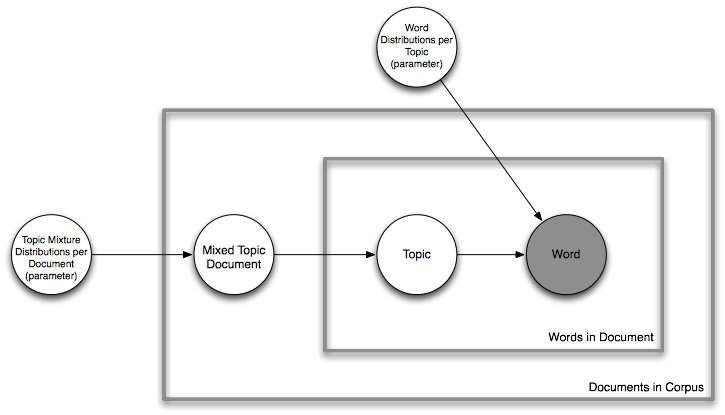
\includegraphics[width=5in]{lda.png}
\caption{A Graphical Model of LDA}
\label{gm_lda}
\end{figure*}

\section{MapReduce for Latent Dirichlet Allocation}

As shown in Table \ref{lda_comp}, a comparison of different approaches for LDA was summarized \cite{zhai2012mr}. From the table, we can see that pLDA, Mahout, and Mr.LDA were implemented in the MapReduce paradigm. 

\begin{table}[!t]
\caption{A comparison of different approaches for LDA}
\label{lda_comp}
\centering
\begin{tabular}{lll}\hline
Approach  & Framework        & Inference                     \\ \hline
Mallet \cite{mallet}   & Multi-thread     & Gibbs                         \\
GPU-LDA \cite{yan2009parallel}   & GPU              & Gibss \& Variational Bayesian \\
Async-LDA \cite{smyth2008asynchronous} & Multi-thread     & Gibbs                         \\
N.C.L. \cite{mariote2007parallelized}   & Master-Slave     & Variational Bayesian          \\
pLDA \cite{wang2009plda}     & MPI \& MapReduce & Gibbs                         \\
Y!LDA \cite{smola2010architecture}    & Hadoop           & Gibbs                         \\
Mahout \cite{mahout_lda}   & MapReduce        & Variational Bayesian          \\
Mr. LDA \cite{zhai2012mr}   & MapReduce        & Variational Bayesian         \\\hline
\end{tabular}
\end{table}

For the implementation of Mahout, it regards the variational inference as a generation of Expectation Maximization (EM) algorithm for hierarchical Bayesian models. Therefore, for the E step, it infers the posterior probability of each topic for each word for all the documents in the collection. Then, it emits the statistics for each word in each topic. For the M step, it sums and normalizes the statistics, therefore we can get the distribution of the corpus for each topic. These two steps were implemented in Mapper and Reducer, respectively \cite{mahout_lda}. 

\begin{algorithm}
\caption{Mapper}
\label{alg:lda_map}
\begin{algorithmic}
\STATE{\textbf{Key} - document ID $d\in \{1,\ldots,D\}$}
\STATE{\textbf{Value} - document content}
\REQUIRE Initialize global parameters $\lambda$
    \FOR{each topic $k$ and word $v$}
	\STATE{$\lambda_{k,v}^{(t+1)}=\eta+\sum_{d=1}^D\sum_{n=1}^N{1(w_{d,n}=v)\phi_{n,k}^{(t)}}$}
	\STATE{\textbf{Emit $\lambda_{k,v}^{(t+1)}$}}
    \ENDFOR
    \FOR{each document $d \in \{1,\ldots,D\}$}
	\STATE{$\gamma_{d,k}^{(t+1)}=\alpha_k+\sum_{n=1}^N{\phi_{d,n,k}^{(t)}}$}
		\FOR{each word $n$}
		\STATE{$\phi_{d,n,k}^{(t+1)} \propto \left\lbrace \Phi(\gamma_{d,k}^{(t+1)})+ \Phi(\lambda_{k,w_n}^{(t+1)})-\Phi(lambda_{k,v}^{(t+1)}) \right\rbrace $}
		\STATE{\textbf{Emit $\phi_{d,n,k}^{(t+1)}$}}
    		\ENDFOR
    		\STATE{\textbf{Emit $\gamma_{d,k}^{(t+1)}$}}
    \ENDFOR
\end{algorithmic}
\end{algorithm}

\begin{algorithm}
\caption{Reducer}
\label{alg:lda_reduce}
\begin{algorithmic}
\STATE{\textbf{Calculate}}
\STATE{$\hat{\beta}_{k,v} = \frac{\lambda}{\sum_{v'=1}^V{\lambda_{k,v'}}}$}
\STATE{$\hat{\theta}_{d,k} = \frac{\gamma_{d,k}}{\sum_{k'=1}^K{\gamma_{d,k'}}}$}
\STATE{$\hat{z}_{d,n,k} = \phi_{d,n,k}$}
\end{algorithmic}
\end{algorithm}

\section{Experiment}
\subsection{Dataset}
The dataset of this project is obtained from Kaggle (www.kaggle.com), which is a platform for data analysis and prediction competitions. The data that we use are posted by Facebook for a keyword extraction competition. The dataset consists the files both for training and testing, of which the training file contains four attributes - id, title, body, and tags. In this project, only the title and body are used to extract the topics. A summary of the dataset is shown as below.
\begin{itemize}
\item Size: 7.3 GB
\item Number of texts: 6,034,195
\item Number of unique tags: 42048
\item Top 10 tags:\\
\begin{verbatim}
c# 463526
java 412189
php 392451
javascript 365623
android 320622
jquery 305614
c++ 199280
python 184928
iphone 183573
asp.net 177334
\end{verbatim}
\end{itemize}
Example:
\begin{quote}

\textbf{id}: 1

\textbf{title}: How to check if an uploaded file is an image without mime type?

\textbf{content}:

I'd like to check if an uploaded file is an image file (e.g png, jpg,  jpeg, gif, bmp) or another file. The problem is that I'm using Uploadify  to upload the files, which changes the mime type and gives a 'text/octal'  or something as the mime type, no matter which file type you upload.


Is there a way to check if the uploaded file is an image apart from checking the file extension using PHP?

\textbf{tags}: php image-processing file-upload upload mime-types
\end{quote}

\subsection{Hadoop Setup}

The hadoop cluster contains six nodes including one masternode and five slavenodes. To set up the hadoop cluster, we first configured the hosts file as shown below.

\begin{verbatim}
192.168.65.70 masternode
192.168.65.71 slavenode1
192.168.65.72 slavenode2
192.168.65.75 slavenode3
192.168.65.76 slavenode4
192.168.65.77 slavenode5
\end{verbatim}

To configure the hadoop accordingly, we updated the \verb+conf/masters+ and \verb+conf/slaves+ files on the master node as shown below.\\[10pt]
\verb+conf/masters+ on the master node:
\begin{verbatim}
masternode
\end{verbatim}\\
\verb+conf/slaves+ one the master node:
\begin{verbatim}
slavenode1
slavenode2
slavenode3
slavenode4
slavenode5
\end{verbatim}

In addition, configuration files \verb+conf/core-site.xml+, \verb+conf/mapred-site.xml+, and \verb+conf/hdfs-site.xml+ were modified on all the nodes as shown below.\\[10pt]
\verb+conf/core-site.xml+ on all the nodes:

\begin{verbatim}
<configuration>
<property>
<name>fs.default.name</name>
<value>hdfs://masternode:9000</value>
<description>Enter your NameNode hostname
</description>
</property>
<property>       
<name>fs.checkpoint.dir</name>       
<value>/home/student/DAT500/fs/hdfs/snn
</value>
<description>A comma separated list of paths.
 Use the list of directories</description>
</property>
<property>       
<name>hadoop.tmp.dir</name>       
<value>/home/student/DAT500/fs/tmp</value>  
<description>Comma separated list of paths
</description>
</property>
</configuration>
\end{verbatim}\\[10pt]
\verb+conf/mapred-site.xml+ on all the nodes:
\begin{verbatim}
<configuration>
<property>
<name>mapred.job.tracker</name>
<value>masternode:9001</value>
<description>Enter your JobTracker hostname
</description>
</property>
<property>       
<name>mapred.local.dir</name>       
<value>/home/student/DAT500/fs/tmp/mapred/
local</value>  
<description>Comma separated list of paths
</description>
</property>
</configuration>
\end{verbatim}\\[10pt]
\verb+conf/hdfs-site.xml+ on all the nodes:
\begin{verbatim}
<configuration>
<property>       
<name>dfs.name.dir</name>       
<value>/home/student/DAT500/fs/hdfs/nn
</value>  
<description>Comma separated list of paths
</description>
</property>
<property>       
<name>dfs.data.dir</name>       
<value>/home/student/DAT500/fs/hdfs/dn
</value>  
<description>Comma separated list of paths
</description>
</property>
<property>
<name>dfs.replication</name>
<value>2</value>
</property>
</configuration>
\end{verbatim}

\subsection{Data Preprocessing}
Due to the nature of the stack overflow platform, the posts come in various forms. Most posts has weird characters, huge amount of numbers and texts that's not natural language, representing mathematical formulations, program codes and also program or compiling outputs. For example, a lot of questions are asked about a certain compilation error or run time error, which very commonly contains a very long sequence of error report such as stack trace. These text do includes huge amount of text however, they're machine generated output and can be very confusing to the LDA training process. Therefore, we perform a certain steps of preprocessing before we actually run LDA. This not only prevent the unneccesary alements of the posts from confusing the training process but also reduce the data size tremendously.

\begin{itemize}
	\item \textbf{Retrieve related fields.} The original data comes in a csv file with four fields for each record: id, title, body, tag. Since we want to find out the popular topics among the posts, we want to use the text-rich segments (title and body). Tag is essentially the topic in a sense (tags are mostly about what technology the post is asking like a certain programming language). This can be used as the gold standard later to evaluate the topics we found. Thus, we eliminate them for the training process. 
	\item \textbf{Remove contents} in \verb+<code></code>+. The \verb+<code></code>+ tag contains a lot of mathematical formulations, machine generated text etc. Since they're not helpful in finding topics, we eliminate them.
	\item \textbf{Remove tags.} Tags like \verb+<p></p>+ have a large frequency whereas they have no contribution to any topics. So they're all removed.
	\item \textbf{Remove punctuations.} Removing punctuations helps greatly with reducing the feature space. If punctuations are not removed, "happy", "happy." and "happy," would be regarded as different words whereas they should be the same.
	\item \textbf{Lowercase the text.} Lowercase the entire text also helps with reducing feature space since otherwise "happy" and "hapPy" would be regarded as different.
	\item \textbf{Remove newlines and excessive white spaces.}. Since the preprocessed text will be fed into mahout later and text is segmented into words by white space in mahout. Therefore, this would guarantee mahout segments words correctly.
\end{itemize}

\subsection{Local Experiment}

Local experiement is a sequential execution of all essential steps. There are three major steps:

\begin{itemize}
	\item \textbf{Preprocessing.} Preprocessing the text with the steps described in the previous section. The output is a single file with individual documents taking one line in the file.
	\item \textbf{LDA input preparation.} Mahout's LDA takes a specific form of input. It comes with a utility to turn a text file into sequence of entries and then process them further into numeric vectors which is the input form of LDA model training. Therefore, the output from the prepocessing step need to be turned into a form of one entry per physical file which is the input format of the utility function of mahout.
	\item \textbf{LDA model training.} After the input of LDA model training is prepared, it is inputed into mahout and an LDA model will be trained. A utility function is provided within mahout to provide transformation from numerical vectors into original words. We wrote a simple function to extract words with the highest scores in each topic and the result is shown in next section.
\end{itemize}

\subsection{Hadoop Experiment}

Hadoop experiment uses MapReduce to do all the three steps in local experiment.

For the preprocessing, since each document is preprocessed in exactly the same way and the preprocessing of each document is independent. Thus, this perfectly fits into MapReduce platform. We adapted the local preprocessing code to fit the MapReduce framework. A mapper takes in a chunck of text, splits it into entries and then preprocess each entry. A sampling is performed during emittion, the reason is explained in results session. We only emit the preprocessed entry by a predefined probability. The reducer putss each entry into a separate file.

For the LDA input preparation and LDA model training, MapReduce framework is already supported in mahout. The only thing difference is we use a different set of commands with hadoop. 
\subsection{Results}

We ran the LDA on the preprocessed text. We do a sampling during preprocessing the text because using all the entries for training a LDA model would be too much both in terms of storage space and also time. Further, according to Blei etc. \cite{blei2003latent}, LDA model performance plateaus with increasing training set size as all other machine learning models. They used 8000 data points and found out the model is trained sufficiently long before using the entire dataset. Therefore, to avoid over-training the model, we randomly sampled 4145 data entry for LDA model training. We present the result for 10 and 20 topics as shown in Table \ref{result1} and Table \ref{result2}, respectively.

\begin{table*}[!t]
\caption{Results of LDA for 10 topics}
\label{result1}
\centering
  \begin{tabular}{ l  l  l }
    \hline
    Topic number & Top 10 words & Topic summary \\ \hline
    1 & time code run test start program process data memory thread & Program testing, measuring \\ 
    2 & page html php form http jquery javascript post url request & Web programing \\ 
    3 & file error code xml line python string script output files  & N/A \\ 
    4 & windows server system version error directory install folder build linux & System programming \\ 
    5 & class object method function array call type return variable instance & OOP \\ 
    6 & number question set amp frac mathbb find int sum point & N/A \\ 
    7 & java server android apache eclipse http sun attrs hibernate jar & Java \\ 
    8 & data database table sql id query list row column mysql & Database \\ 
    9 & view image button text images display click background menu layout & HTML programming \\ 
    10 & user app application server api client google access facebook & App \\
    \hline
  \end{tabular}
\end{table*}

\begin{table*}[!t]
\caption{Results of LDA for 20 topics}
\label{result2}
\centering
\begin{tabular}{ll}\hline
Topic number & Topic words                                                                                                                                        \\\hline
1            & server client network connection ip remote machine connect domain windows internet port access host set running servers address problem            \\
2            & application project xml web code android app library net build studio visual file system ui development source dll solution                        \\
3            & class object method type function code instance objects call create called methods variable classes context properties variables reference created \\
4            & image images star problem repository size pdf solution svn show git bar don add epsilon http photo png merge                                       \\
5            & button form user event click code list control tab item add selected menu text page change select input custom                                     \\
6            & frac mathbb sum amp attrs matrix function left times question show int vector points set space text order end                                      \\
7            & time process memory thread run application start running code device stop task mode app android threads long service play                          \\
8            & page html php jquery javascript code http ajax content pages css js link post function url plugin working work                                     \\
9            & windows test install version run bit ve installed system running package cache dev rails os fine tests unit ubuntu                                 \\
10           & java org server apache sun impl core eclipse hibernate http jar invoke tomcat jersey postgresql rules loader lang method                           \\
11           & table database sql data query id column mysql row tables db columns category order rows update insert server select                                \\
12           & error code message service exception problem send call email fine works ve wrong string return mail case returns function                          \\
13           & data time date store ve format save read customer correct location appreciated report json field sort point back convert                           \\
14           & group node child number root set language add graph filter good book attributes list attribute xxxxxxxx tree lt english                            \\
15           & question ve find make don good problem simple time lot found answer questions work solution bit idea thing edit                                    \\
16           & array string code function values number python variable loop key numbers simple characters output return find result input replace                \\
17           & file files command script directory error folder line program copy run output work path found python read doesn windows                            \\
18           & user web app api request login users google site http facebook session access password application url create post browser                         \\
19           & view method app controller model iphone set action remove length ios object null code failed mvc check nbsp problem                                \\
20           & screen text layout code background left change color display problem top bar line content cell don width image size  \\ \hline                             
\end{tabular}
\end{table*}
% An example of a floating figure using the graphicx package.
% Note that \label must occur AFTER (or within) \caption.
% For figures, \caption should occur after the \includegraphics.
% Note that IEEEtran v1.7 and later has special internal code that
% is designed to preserve the operation of \label within \caption
% even when the captionsoff option is in effect. However, because
% of issues like this, it may be the safest practice to put all your
% \label just after \caption rather than within \caption{}.
%
% Reminder: the "draftcls" or "draftclsnofoot", not "draft", class
% option should be used if it is desired that the figures are to be
% displayed while in draft mode.
%
%\begin{figure}[!t]
%\centering
%\includegraphics[width=2.5in]{myfigure}
% where an .eps filename suffix will be assumed under latex, 
% and a .pdf suffix will be assumed for pdflatex; or what has been declared
% via \DeclareGraphicsExtensions.
%\caption{Simulation Results}
%\label{fig_sim}
%\end{figure}

% Note that IEEE typically puts floats only at the top, even when this
% results in a large percentage of a column being occupied by floats.


% An example of a double column floating figure using two subfigures.
% (The subfig.sty package must be loaded for this to work.)
% The subfigure \label commands are set within each subfloat command, the
% \label for the overall figure must come after \caption.
% \hfil must be used as a separator to get equal spacing.
% The subfigure.sty package works much the same way, except \subfigure is
% used instead of \subfloat.
%
%\begin{figure*}[!t]
%\centerline{\subfloat[Case I]\includegraphics[width=2.5in]{subfigcase1}%
%\label{fig_first_case}}
%\hfil
%\subfloat[Case II]{\includegraphics[width=2.5in]{subfigcase2}%
%\label{fig_second_case}}}
%\caption{Simulation results}
%\label{fig_sim}
%\end{figure*}
%
% Note that often IEEE papers with subfigures do not employ subfigure
% captions (using the optional argument to \subfloat), but instead will
% reference/describe all of them (a), (b), etc., within the main caption.


% An example of a floating table. Note that, for IEEE style tables, the 
% \caption command should come BEFORE the table. Table text will default to
% \footnotesize as IEEE normally uses this smaller font for tables.
% The \label must come after \caption as always.
%
%\begin{table}[!t]
%% increase table row spacing, adjust to taste
%\renewcommand{\arraystretch}{1.3}
% if using array.sty, it might be a good idea to tweak the value of
% \extrarowheight as needed to properly center the text within the cells
%\caption{An Example of a Table}
%\label{table_example}
%\centering
%% Some packages, such as MDW tools, offer better commands for making tables
%% than the plain LaTeX2e tabular which is used here.
%\begin{tabular}{|c||c|}
%\hline
%One & Two\\
%\hline
%Three & Four\\
%\hline
%\end{tabular}
%\end{table}


% Note that IEEE does not put floats in the very first column - or typically
% anywhere on the first page for that matter. Also, in-text middle ("here")
% positioning is not used. Most IEEE journals/conferences use top floats
% exclusively. Note that, LaTeX2e, unlike IEEE journals/conferences, places
% footnotes above bottom floats. This can be corrected via the \fnbelowfloat
% command of the stfloats package.



\section{Conclusion}
In this project, we studied Latent Dirichlet Allocation using MapReduce. An experiment was conducted to discover the underlying topics of Stackoverflow using LDA. The results showed that LDA successfully extracted some interesting topics.




% conference papers do not normally have an appendix


% use section* for acknowledgement
%\section*{Acknowledgment}




% trigger a \newpage just before the given reference
% number - used to balance the columns on the last page
% adjust value as needed - may need to be readjusted if
% the document is modified later
%\IEEEtriggeratref{8}
% The "triggered" command can be changed if desired:
%\IEEEtriggercmd{\enlargethispage{-5in}}

% references section

% can use a bibliography generated by BibTeX as a .bbl file
% BibTeX documentation can be easily obtained at:
% http://www.ctan.org/tex-archive/biblio/bibtex/contrib/doc/
% The IEEEtran BibTeX style support page is at:
% http://www.michaelshell.org/tex/ieeetran/bibtex/
%\bibliographystyle{IEEEtran}
% argument is your BibTeX string definitions and bibliography database(s)
%\bibliography{IEEEabrv,../bib/paper}
%
% <OR> manually copy in the resultant .bbl file
% set second argument of \begin to the number of references
% (used to reserve space for the reference number labels box)

\bibliography{ref}
\bibliographystyle{plain}



% that's all folks
\end{document}


